\documentclass[12pt]{article}
\usepackage{ficha}

\begin{document}

\ficha{Isometrias, Simetrias e Vetores}[Reflexão, Rotação, Translação e Reflexão Deslizante]

\instrucoes{Resolve os exercícios. Usa papel quadriculado sempre que precisares de construir figuras.}

\secao{Eixos de Simetria}{Indica o número de eixos de simetria de cada figura.}
\begin{exercicios}
  \item Um quadrado.
  \item Um retângulo (não quadrado).
  \item Um triângulo equilátero.
  \item Um triângulo isósceles (não equilátero).
  \item Um losango (não quadrado).
  \item Um paralelogramo (não retângulo nem losango).
  \item Um hexágono regular.
  \item Uma circunferência.
  \item Quais das letras A, H, N, S, T, X, Z têm pelo menos um eixo de simetria?
  \item Quais das letras A, H, N, S, T, X, Z têm simetria de rotação?
\end{exercicios}

\secao{Reflexão}{Observa a figura e responde.}

\begin{center}
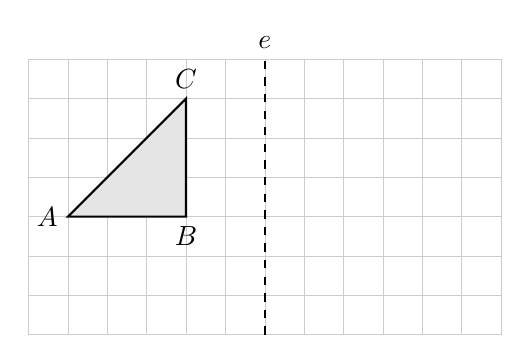
\begin{tikzpicture}[scale=0.5]
  \draw[very thin, gray!40] (-6,-3) grid (6,4);
  \draw[thick, dashed] (0,-3) -- (0,4) node[above] {$e$};
  \draw[thick, fill=gray!20] (-5,0) node[left] {$A$} -- (-2,0) node[below] {$B$} -- (-2,3) node[above] {$C$} -- cycle;
\end{tikzpicture}
\end{center}

\begin{exercicios}
  \item Desenha a imagem do triângulo $ABC$ pela reflexão de eixo $e$.
  \item A imagem tem a mesma forma e o mesmo tamanho que a figura original? Como se chama uma transformação com esta propriedade?
  \item A que distância do eixo fica a imagem de $A$? E a de $B$?
  \item Num referencial, indica a imagem do ponto $(3, 5)$ pela reflexão de eixo $Oy$.
  \item Indica a imagem do ponto $(3, 5)$ pela reflexão de eixo $Ox$.
  \item Indica a imagem do ponto $(-2, 4)$ pela reflexão de eixo $y = x$.
\end{exercicios}

\secao{Rotação}{Resolve. Considera o sentido positivo como o sentido contrário ao dos ponteiros do relógio.}
\begin{exercicios}
  \item Indica a imagem do ponto $(4, 0)$ pela rotação de centro $O$ e amplitude $90^\circ$.
  \item Indica a imagem do ponto $(2, 3)$ pela rotação de centro $O$ e amplitude $180^\circ$.
  \item Indica a imagem do ponto $(1, 5)$ pela rotação de centro $O$ e amplitude $-90^\circ$.
  \item Um quadrado roda em torno do seu centro. Para que amplitudes (entre $0^\circ$ e $360^\circ$) a imagem coincide com o quadrado?
  \item Qual é a menor amplitude de rotação que faz coincidir um hexágono regular consigo próprio?
  \item Qual é a menor amplitude de rotação que faz coincidir um triângulo equilátero consigo próprio?
  \item Uma rotação de $360^\circ$ é equivalente a que transformação?
\end{exercicios}

\secao{Vetores e Translações}{Responde a cada questão.}

\begin{center}
\begin{tikzpicture}[scale=0.55]
  \draw[very thin, gray!40] (0,0) grid (12,6);
  \draw[-{Latex}, thick] (1,1) -- (4,3) node[midway, above left] {$\vec u$};
  \draw[-{Latex}, thick] (6,5) -- (8,1) node[midway, right] {$\vec v$};
  \draw[-{Latex}, thick] (9,2) -- (12,4) node[midway, above left] {$\vec w$};
  \draw[-{Latex}, thick] (2,5) -- (5,5) node[midway, above] {$\vec a$};
\end{tikzpicture}
\end{center}

\begin{exercicios}
  \item Indica dois vetores iguais. Justifica.
  \item Indica a direção, o sentido e o comprimento (em quadrículas) de $\vec a$.
  \item Desenha um vetor simétrico de $\vec v$.
  \item Desenha o vetor $\vec u + \vec a$.
  \item Num referencial, indica a imagem do ponto $(2, 1)$ pela translação de vetor $(3, -4)$.
  \item O ponto $P'(5, 7)$ é a imagem de $P$ pela translação de vetor $(2, 3)$. Determina $P$.
  \item Que translação transforma o ponto $(1, 2)$ no ponto $(-3, 6)$?
  \item Aplica sucessivamente as translações de vetores $(2, 1)$ e $(-5, 3)$ ao ponto $(0, 0)$. Que translação única é equivalente?
\end{exercicios}

\secao{Composição de Isometrias}{Responde a cada questão.}
\begin{exercicios}
  \item O que é uma reflexão deslizante? Dá um exemplo do dia a dia.
  \item Aplica ao ponto $(2, 3)$ a reflexão de eixo $Ox$ seguida da translação de vetor $(4, 0)$. Qual é a imagem final?
  \item Aplica duas reflexões sucessivas de eixos paralelos $x = 1$ e $x = 4$ ao ponto $(0, 2)$. Que transformação única é equivalente?
  \item Aplica duas reflexões sucessivas de eixos $Ox$ e $Oy$ ao ponto $(3, 1)$. Que transformação única é equivalente?
  \item Indica uma isometria que transforma o segmento de extremos $(0,0)$ e $(2,0)$ no segmento de extremos $(0,0)$ e $(0,2)$.
\end{exercicios}

\secao{Desafios}{Resolve os problemas.}
\begin{exercicios}
  \item Um friso é um padrão que se repete ao longo de uma faixa. Desenha um friso que tenha simetria de translação e de reflexão de eixo vertical.
  \item Um polígono regular tem simetria de rotação de $40^\circ$. Quantos lados tem?
  \item O triângulo de vértices $A(1, 1)$, $B(4, 1)$ e $C(1, 3)$ sofre uma rotação de $90^\circ$ em torno de $A$. Determina as imagens de $B$ e $C$.
  \item Explica por que razão as isometrias preservam a área das figuras.
  \item Uma rosácea tem 5 eixos de simetria. Quais são as amplitudes das rotações que o deixam invariante?
\end{exercicios}

\end{document}
